%% ****** Start of file apstemplate.tex ****** %
%%
%%
%%   This file is part of the APS files in the REVTeX 4.2 distribution.
%%   Version 4.2a of REVTeX, January, 2015
%%
%%
%%   Copyright (c) 2015 The American Physical Society.
%%
%%   See the REVTeX 4 README file for restrictions and more information.
%%
%
% This is a template for producing manuscripts for use with REVTEX 4.2
% Copy this file to another name and then work on that file.
% That way, you always have this original template file to use.
%
% Group addresses by affiliation; use superscriptaddress for long
% author lists, or if there are many overlapping affiliations.
% For Phys. Rev. appearance, change preprint to twocolumn.
% Choose pra, prb, prc, prd, pre, prl, prstab, prstper, or rmp for journal
%  Add 'draft' option to mark overfull boxes with black boxes
%  Add 'showkeys' option to make keywords appear
%\documentclass[aps,prl,preprint,groupedaddress]{revtex4-2}
%\documentclass[aps,prl,preprint,superscriptaddress]{revtex4-2}
%\documentclass[aps,prl,reprint,groupedaddress]{revtex4-2}
\documentclass[aps,prb,reprint,superscriptaddress]{revtex4-2}

\usepackage{blindtext}
\usepackage{mhchem}
\usepackage{hyperref}
\usepackage{bm}
\usepackage{siunitx}
\usepackage{mathrsfs}
\usepackage{csquotes}

\graphicspath{{source/}}

% You should use BibTeX and apsrev.bst for references
% Choosing a journal automatically selects the correct APS
% BibTeX style file (bst file), so only uncomment the line
% below if necessary.
%\bibliographystyle{apsrev4-2}

\begin{document}

% Use the \preprint command to place your local institutional report
% number in the upper righthand corner of the title page in preprint mode.
% Multiple \preprint commands are allowed.
% Use the 'preprintnumbers' class option to override journal defaults
% to display numbers if necessary
%\preprint{}

%Title of paper
\title{Self-organized criticality}

% repeat the \author .. \affiliation  etc. as needed
% \email, \thanks, \homepage, \altaffiliation all apply to the current
% author. Explanatory text should go in the []'s, actual e-mail
% address or url should go in the {}'s for \email and \homepage.
% Please use the appropriate macro foreach each type of information

% \affiliation command applies to all authors since the last
% \affiliation command. The \affiliation command should follow the
% other information
% \affiliation can be followed by \email, \homepage, \thanks as well.
\author{Bryan T. Fichera}
\affiliation{Department of Physics, Massachusetts Institute of Technology, Cambridge, Massachusetts 02139, USA}
\email[]{bfichera@mit.edu}
%\homepage[]{Your web page}
%\thanks{}
%\altaffiliation{}

%Collaboration name if desired (requires use of superscriptaddress
%option in \documentclass). \noaffiliation is required (may also be
%used with the \author command).
%\collaboration can be followed by \email, \homepage, \thanks as well.
%\collaboration{}
%\noaffiliation

\date{\today}

\begin{abstract}
% insert abstract here
\blindtext
\end{abstract}

% insert suggested keywords - APS authors don't need to do this
%\keywords{}

%\maketitle must follow title, authors, abstract, and keywords
\maketitle

\section{Introduction}

A key aspect of the types of phase transitions that we have covered in 8.334 was the concept of a critical point. A system at its critical point is characterized by total scale invariance, in the sense that its relevant correlation lengths are divergent and its correlation functions decay like power laws with separation. The concept of scale invariance was used to illuminate the notion of universality, i.e. the experimental fact that disparate systems with tangible microscopic differences behaved the same way (in the sense of macroscopic observables scaling equivalently with temperature) near the critical point. The critical point itself was found to be a single point or line in the space of the tuning parameters, but an entire volume (with codimension equivalent to the number of tuning parameters) in the space of all parameters (both microscopic and macroscopic) relevant to the system.

In the systems that we considered in class, to reach a critical point it was necessary to drive the system by some combination of external parameters like temperature, pressure, or magnetic field. In addition, the critical point was always unstable to small fluctuations in the tuning parameters, so that a state of persistent criticality was practicallyimpossible. While this is certainly characteristic of the majority of physical systems in the everyday world, there are in fact a variety of other systems for which criticality -- in the sense of divergent correlation lengths, power law decay of correlation functions, and inherent scale invariance -- is rather an emergent property, which arises naturally without any fine-tuning of experimental parameters. This phenomenon has been called ``self-organized criticality'' (SOC), and is thought to underpin the physics of a number of natural critical phenomena such as earthquakes, forest fires, and droplet formation, which display critical behavior in the absence of tuning parameters.

In this term paper, I discuss a simple lattice model exhibiting SOC known as the Abelian sandpile model (ASM). First I give a brief overview of the ASM, including a discussion of the critical phenomenology. Then, to connect the ASM with the lattice models which we discussed in class, I reproduce the proof that the ASM is equivalent to the $q \rightarrow 0$ limit of the Potts model, which was given by Majumdar and Dhar in 1992~\cite{majumdar_equivalence_1992}. To conclude the paper, I discuss the effects of finite temperature on so-called "hot" sandpiles~\cite{caldarelli_hot_1996}, and with simulations describe the effect of temperature on a related model of my own construction.

\section{The abelian sandpile model}

\subsection{Definition\label{sec:rules}}

The ASM was discovered in 1987 by Bak, Tang, and Wiesenfeld as the first example of a dynamical system exhibiting self-organized criticality~\cite{bak_self-organized_1987}. At a schematic level, the model consists of a $d$-dimensional lattice whose sites are described as containing an integer number of grains of sand. At any given site, if the number of grains is greater than some threshold value then the site ``topples,'' scattering its sand to its nearest neighbors. A single step of the evolution of the system consists of randomly adding one grain of sand to the lattice, and then relaxing the system by some defined toppling rules. After the system is stable with respect to those toppling rules, then another grain of sand is added to a random site and the evolution continues. In this respect, the drive frequency of the ASM is said to be much smaller than the relaxation rate.

Mathematically, the ASM can be defined as follows. Let $z_i$ be the number of grains at site $i$, $1 \leq i \leq N$ on a given lattice with $N$ sites, and let each site be assigned a threshold value $\Delta_{ii}$. Then evolve the system according to the following rules:

\begin{enumerate}
\item[(i)] Choose an integer $i$ randomly from $[1, N]$. Take $z_i \rightarrow z_i+1$.
\item[(ii)] For each $j$ such that $z_j \geq \Delta_{jj}$, perform a topple at site $j$ according to the toppling rule:
\begin{enumerate}
\item[(i.a)] For each integer $k \in [1, N]$, take $z_k \rightarrow z_k - \Delta_{jk}$.
\end{enumerate}
\item[(iii)] Repeat (ii) until there are no integers $j$, $1 \leq j \leq N$ such that $z_j \geq \Delta_{jj}$.
\item[(iv)] Repeat from (i).
\end{enumerate}

An additional requirement of the ASM is that the system lose some amount of sand to dissipation, or else continual evolution of the system will result in a state with high density and infinite toppling time. Note that with this condition, $\sum_j\Delta_{ij} \geq 0$ for all $i$. Dissipation is typically introduced using so-called open boundary conditions, where the sandpile is said to exist on a table such that grains of sand can topple over the edge, where they disappear.

An illustration of a simple 2-dimensional ASM is given in Fig.~\ref{fig:rules}. It can be shown~\cite{dhar_self-organized_1990} that the toppling rules described above give rise to relaxation rules that are abelian, in the sense that a state where multiple sites are above the threshold will always relax to the same final state, regardless of the order in which the critical sites are toppled.

\begin{figure}
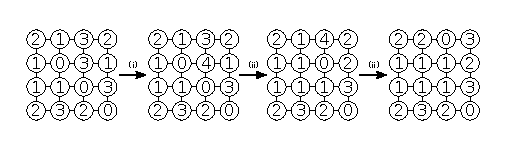
\includegraphics{rules}
\caption{\label{fig:rules} An illustration of the ASM toppling rules (section~\ref{sec:rules}) in the simple case of a $4 \times 4$ square lattice with open boundary conditions, with $\Delta_{ij} = -1$ if sites $i$ and $j$ are nearest neighbors, $\Delta_{ij} = 4$ if $i = j$, and $\Delta_{ij} = 0$ otherwise.}
\end{figure}

\subsection{Phenomenology}

In the ASM, there are in general three quantities which are used to study the dynamical properties. First, define for a given avalanche

\begin{enumerate}
\item[(i)] $n$, the number of topples involved in the avalanche before the system relaxes to a stable state,
\item[(ii)] $t$, the number of time steps required for the relaxation process (the ``lifetime'' of the avalanche),
\item[(iii)] $l$, the linear size of the avalanche, 
\[
l = \dfrac{1}{|A|}\sum_i|\bm{r}-\bm{R}_{cm}|,
\]
where
\[
\bm{R}_{cm} = \dfrac{1}{|A|}\sum_i\bm{r}_i.
\]
\end{enumerate}

Of course the above quantities are not independent, so to discuss the statistical nature of the system it is necessary to study the joint probability distribution for avalanches $P(n, t, l)$. However, this is computationally quite difficult so that researchers mostly study the unconditional probability distributions $P(n)$, $P(t)$, and $P(l)$, where $P(x)$ is the probability that a given avalanche has property $x$, irrespective of the other two quantities. The ASM is said to exhibit self-organized criticality because the probabilities $P(n)$, $P(t)$, and $P(l)$ are power law distributed in their arguments~\cite{jensen}.

To show that the ASM exhibits self-organized criticality, I performed simulations of an ASM on a 2-dimensional $20 \times 20$ square lattice with open boundary conditions, nearest-neighbor toppling rules like those in Fig.~\ref{fig:rules}, and $\Delta_{ii} = 4$ for all $i$. Histograms of avalanche sizes and lifetimes in the simulation are plotted in Fig.~\ref{fig:avalanches}(a) and (b), respectively.

\begin{figure}
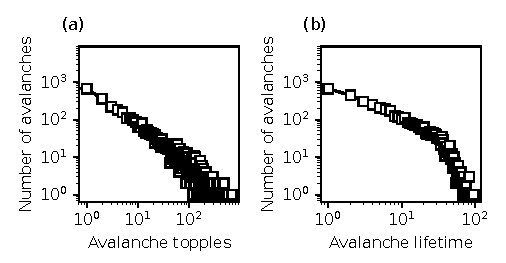
\includegraphics{avalanches}
\caption{\label{fig:avalanches}Histogram of avalanche sizes, $n$ (a) and avalanche lifetimes, $t$ (b) after $10000$ drive periods on a 2-dimensional $20 \times 20$ square ASM model with open boundary conditions, nearest-neighbor toppling rules like Fig.~\ref{fig:rules}, and $\Delta_{ii} = 4$ for all $i$. The histograms show power law behavior over 1-2 decades. Deviations from power law behavior are likely due to finite-size effects~\cite{jensen}.}
\end{figure}








\bibliography{asm}

\end{document}
